\subsection{Тестирование}

\subsubsection{Метод прогонки}

Нижняя и верхняя диагональ заполняются случайными числами. Главная диагональ заполняется следующим образом:
\[
  c_i = \left\lvert a_i \right\rvert + \left\lvert b_i \right\rvert + 1
\]
Главная диагональ заполняется таким образом для уменьшения возможности появления плохо обусловленной матрицы.
Также случайными числами заполняется вектор решения $ x $.

Чтобы получить вектор $ g $, мы умножаем матрицу на вектор решения. После получения вектора $ g $
используем наш метод прогонки, чтобы получить вектор решения $ \tilde{x} $. Для прохождения теста, полученные данные должны
соответствовать следующему неравенству:
\[
  \left\lVert \tilde{x} - x \right\rVert < cond(A) \varepsilon_M \left\lVert x \right\rVert 
\]
Результат выполнения тестов:
\begin{center}
  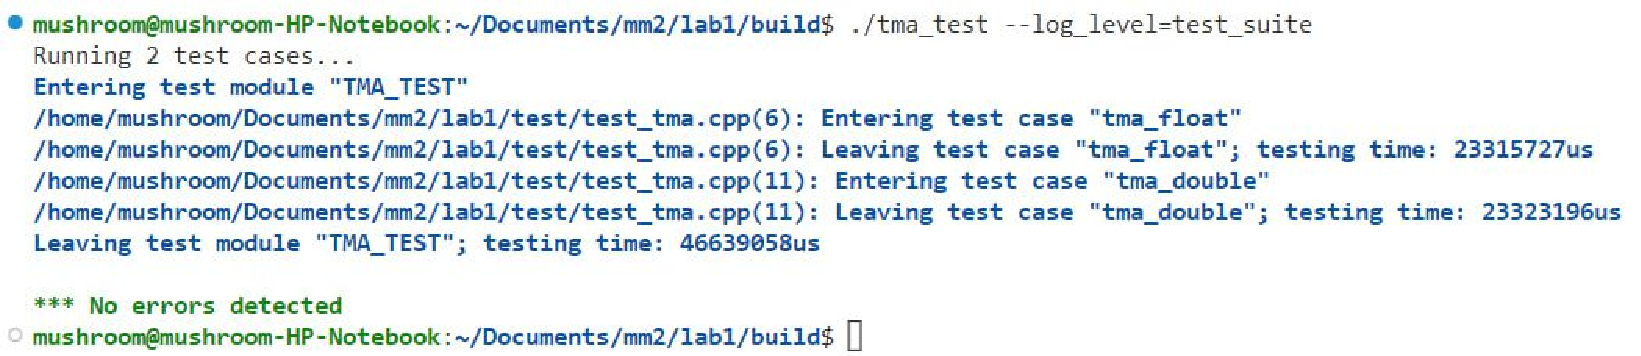
\includegraphics[width=\textwidth]{img/test.pdf}
\end{center}

\subsubsection{Интегро-интерполяционный метод}

Выполним нашу программу на ряде входных параметров

\begin{table}[H]
  \centering
  \begin{tabular}{ c | *{8}c }
    \toprule
    Номер теста & k & q & u & f & $\nu_1 $ & $\nu_2 $ & $R_L$ & $R_R$\\
    \midrule
    1 & r & 1 & 2r + 3 & 2r - 1 & -2 & 4 & 1 & 2 \\
    \midrule
    2 & $r^2$ & 1 & $2r^2 + 3$ & $-14r^2 + 3$ & -4 & 32 & 1 & 2 \\
    \midrule
    3 & $r^3$ & 1 & $2r^3 + 3$ & $-36r^4 + 2r^3 + 3$ & -6 & 192 & 1 & 2 \\
    \bottomrule
  \end{tabular}
\end{table}

После запуска программы мы получаем следующие результаты:
  \begin{table}[H]
    \centering
    \begin{tabular}{c | c | c}
      \toprule
      N & $ \left\lVert \varepsilon \right\rVert  $, одинарная точность & $ \left\lVert \varepsilon \right\rVert  $, двойная точность \\
      \midrule
      8 & 2.45905e-03 & 2.46952e-03\\
      16 & 6.10828e-04 & 6.19519e-04\\
      32 & 1.39713e-04 & 1.55015e-04\\
      64 & 6.91414e-05 & 3.87621e-05\\
      128 & 6.19888e-05 & 9.69106e-06\\
      256 & 2.66743e-03 & 2.42279e-06\\
      512 & 9.03511e-03 & 6.05706e-07\\
      1024 & 9.06944e-03 & 1.51435e-07\\
      2048 & 4.98871e-01 & 3.78822e-08\\
      \bottomrule
    \end{tabular}
    \caption{Погрешность теста №1}
  \end{table}

  \begin{table}[H]
    \centering
    \begin{tabular}{c | c | c}
      \toprule
      N & $ \left\lVert \varepsilon \right\rVert  $, одинарная точность & $ \left\lVert \varepsilon \right\rVert  $, двойная точность \\
      \midrule
      8 & 1.49273e-01 & 1.49265e-01\\
      16 & 3.73564e-02 & 3.73383e-02\\
      32 & 9.32503e-03 & 9.33596e-03\\
      64 & 1.68228e-03 & 2.33408e-03\\
      128 & 1.65176e-03 & 5.83525e-04\\
      256 & 1.83487e-03 & 1.45882e-04\\
      512 & 2.59638e-02 & 3.64704e-05\\
      1024 & 7.11317e-01 & 9.11763e-06\\
      2048 & 5.93484 & 2.27931e-06\\
      \bottomrule
    \end{tabular}
    \caption{Погрешность теста №2}
  \end{table}

  \begin{table}[H]
    \centering
    \begin{tabular}{c | c | c}
      \toprule
      N & $ \left\lVert \varepsilon \right\rVert  $, одинарная точность & $ \left\lVert \varepsilon \right\rVert  $, двойная точность \\
      \midrule
      8 & 2.52285 & 2.52289\\
      16 & 6.31502e-01 & 6.31225e-01\\
      32 & 1.5601e-01 & 1.57838e-01\\
      64 & 4.27036e-02 & 3.94614e-02\\
      128 & 1.83411e-02 & 9.86546e-03\\
      256 & 7.73621e-03 & 2.46637e-03\\
      512 & 2.19547e-01 & 6.16594e-04\\
      1024 & 1.32325 & 1.54148e-04\\
      2048 & 17.763 & 3.85369e-05\\
      \bottomrule
    \end{tabular}
    \caption{Погрешность теста №3}
  \end{table}

  Добавим еще один тест
  \begin{align*}
    k &= \frac{\ln(r)}{r} \quad q = \cos(r) \quad u = \sin(r) \\
    r &\in [\frac{\pi}{6}; \frac{\pi}{3} ]
  \end{align*}

  Находим значение $f$ как:
  \[
    -\left[ \frac{1}{r} \frac{d}{dr} \left(r \cdot \frac{\ln(r)}{r} \cdot \frac{d \sin(r)}{dr} \right)\ -\ \cos(r) \cdot \sin(r) \right] = f(r),
  \]

  Получаем:
  \[
    f(r) = -\frac{\cos(r) - r\ln(r)\cdot\sin(r)}{r^2} + \cos(r)\sin(r)
  \]

  Находим значения $ \nu_1 $ и $ \nu_2 $:
  \begin{align*}
		& \frac{\ln(r)}{r} \left. \frac{d\sin(r)}{dr}\right\vert_{r = \frac{\pi}{6}} = -\nu _1
		&-\frac{\ln(r)}{r} \left. \frac{d\sin(r)}{dr}\right\vert_{r = \frac{\pi}{3}} = -\nu_2 \\
    & \nu_1 = -\frac{\ln(\frac{\pi}{6}) \cdot 3\sqrt{3}}{\pi} \\
    &\nu_2 = \frac{\ln(\frac{\pi}{3})\cdot3}{2 \cdot \pi}
  \end{align*}
  \begin{table}[H]
    \centering
    \begin{tabular}{c | c | c}
      \toprule
      N & $ \left\lVert \varepsilon \right\rVert  $, одинарная точность & $ \left\lVert \varepsilon \right\rVert  $, двойная точность \\
      \midrule
      8 & 5.99104e-3 & 5.99104e-3\\
      16 & 1.614304e-3 & 1.614304e-3\\
      32 & 5.16205e-4 & 5.16205e-4\\
      64 & 1.10805e-4 & 1.36056e-4\\
      128 & 3.13878e-4 & 5.854e-05\\
      256 & 8.02338e-4 & 1.19619e-05\\
      512 & 2.43866e-3 & 3.43873e-06\\
      1024 & 1.43307e-2 & 1.16275e-06\\
      2048 & 0.451278 & 1.84805e-07\\
      \bottomrule
    \end{tabular}
    \caption{Погрешность теста №4}
  \end{table}

На данных тестах можно проследить зависимость погрешности от числа разбиений, которую мы выявили в предыдущей главе, что при увеличении шага
в 2 раза погрешность должна уменьшаться примерно в 4 раза. Также можно проследить что есть число разбиений при котором погрешность минимальна.
При дальнейшем увеличении числа разбиений погрешность увеличивается (данное явление можно заметить на тестах одинарной точности).